% \pagebreak[4]
% \hspace*{1cm}
% \pagebreak[4]
% \hspace*{1cm}
% \pagebreak[4]

\chapter{Geometrical Algorithms}
\ifpdf
    \graphicspath{{Chapter1/Chapter1Figs/PNG/}{Chapter1/Chapter1Figs/PDF/}{Chapter1/Chapter1Figs/}}
\else
    \graphicspath{{Chapter1/Chapter1Figs/EPS/}{Chapter1/Chapter1Figs/}}
\fi


\nomenclature[H]{$H$}{ A list of points which denotes potential robot positions.}                  

\nomenclature[Pmaj]{$P_{maj}$}{The majority rule map of all translates of the polygon. The
translates of the polygon are obtained by choosing one hypothesis as the origin and
translating all the remaining hypotheses to this chosen origin.}                               

\nomenclature[Gij]{$G_{ij}$}{ For the translates corresponding to pair of hypotheses $h_{i}$ and
 $h_{j}$, $G_{ij}$ is the origin containing region obtained by taking the lower
envelope of visibility polygons of all type 1 and type 2 edges of the polygon.\\
An edge is of type 1 or type 2, if it belongs to exactly one of the translates.
}                         

\nomenclature[gi]{$g_{i}$}{The set of all points at which $h_{i}$ does not share the majority
opinion about $i$.}          

\nomenclature[Ki]{$K_{i}$}{The majority rule map of $G_{ij}$'s for a particular i and $j \belongs [1...n]\backslash i$}  
\nomenclature[Maj(gamma)]{$Maj(\gamma)$}{Set of hypothesis which share the majority opinion about $\gamma$.
 $\gamma$ can be either a point or a region.} 


\section{Computing Visibility Polygons}
Visibility polygon is an indispensable component in the hypothesis generation step of the algorithm. Since CGAL had no inbuilt support
 for computing visibility polygons we implemented the following two routines for our purposes.
\begin{itemize}
 \item Visibility Polygon of a point inside a polygon
 \item Visibility Polygon of an edge of the polygon.
\end{itemize}


%Java2TeX style definitions
%You can modify them to fit your needs
\newcommand{\jttstylea}{\color[rgb]{1.00,1.00,1.00}} %Background
\newcommand{\jttstyleb}{\color[rgb]{.501,.501,.501}} %Line numbers
\newcommand{\jttstylec}{\color[rgb]{.247,.498,.372}} %Multi-line comments
\newcommand{\jttstyled}{\color[rgb]{.247,.498,.372}} %Single-line comments
\newcommand{\jttstylee}{\color[rgb]{.498,.000,.333}} %Keywords
\newcommand{\jttstylef}{\color[rgb]{.164,.000,1.00}} %Strings
\newcommand{\jttstyleg}{\color[rgb]{.600,.000,.000}} %Character constants
\newcommand{\jttstyleh}{\color[rgb]{.600,.000,.000}} %Numeric constants
\newcommand{\jttstylei}{\color[rgb]{.000,.000,.000}} %Parenthesis
\newcommand{\jttstylej}{\color[rgb]{.498,.000,.333}} %Primitive Types
\newcommand{\jttstylek}{\color[rgb]{.000,.000,.000}} %Others
\newcommand{\jttstylel}{\color[rgb]{.498,.623,.749}} %Javadoc keywords
\newcommand{\jttstylem}{\color[rgb]{.498,.498,.623}} %Javadoc HTML tags
\newcommand{\jttstylen}{\color[rgb]{.247,.247,.749}} %Javadoc links
\newcommand{\jttstyleo}{\color[rgb]{.247,.372,.749}} %Javadoc others
\newcommand{\jttstylep}{\color[rgb]{1.00,.380,.000}} %Undefined
\newcommand{\jttstyleq}{\color[rgb]{.392,.392,.392}} %Annotation


\subsection{Visibility Polygon of a Point Inside a Polygon}

\begin{definition}
 {\bf Visibility Polygon of Point:} $p$ is the bounded polygonal region of all points of the polygon visible from $p$.  
\end{definition}

The following is the C++ function in the file PolygonUtil.cpp. We pass the map polygon and the point $P$, whose visibility polygon is to be
 computed. The function returns the visibility polygon of $P$ as another Polygon type.
In $setVisiblePoints$ we collect all those points which are directly visible from $P$. Note that
 all these points will form a part of the visibility polygon of $P$ since they are directly visible from $P$. These points can contain 
 some reflex vertices as well. A reflex vertex occludes a portion of map resulting in a spurious vertex [\cite{key4}]. Each spurious vertex which is a part of the visibility polygon
 can be obtained by extending the line joining the point $P$ to a reflex vertex. We do this in the if block and collect all the 
spurious vertices also. Finally we sort all the vertices obtained by traversing along the boundary of the map in anticlockwise direction to get the visibility polygon of $P$.\\ \\

{
\noindent \ttfamily
\jttstylek Polygon~PolygonUtil::CalcVisibilityPolygon\jttstylei (\jttstylek Polygon\&~map,~Point\&~point\jttstylei )\\
\jttstylei \{\\
\jttstylea ~~\jttstylek Polygon~setVisiblePoints~=~VisiblePointSet\jttstylei (\jttstylek map,point\jttstylei )\jttstylek ;\\
\jttstylea ~~\jttstylek list\verb#<#Point\verb#>#~listVisiblePoints;\\
\jttstylea \\
\jttstylea ~~\jttstylee for~\jttstylei (\jttstylek VertexIterator~vi~=~setVisiblePoints.vertices\verb#_#begin\jttstylei ()\jttstylek ;~vi~!=~setVisiblePoints.vertices\verb#_#end\jttstylei ()\jttstylek ;~++vi\jttstylei )\\
\jttstylea ~~\jttstylei \{\\
\jttstylea ~~~~\jttstylek listVisiblePoints.push\verb#_#back\jttstylei (\jttstylek \verb#*#vi\jttstylei )\jttstylek ;\\
\jttstylea ~~~~\jttstylee if\jttstylei (\jttstylek IsReflex\jttstylei (\jttstylek map,\verb#*#vi\jttstylei ))\\
\jttstylea ~~~~\jttstylei \{\\
\jttstylea ~~~~~~\jttstylek Ray~rayToCorner\jttstylei (\jttstylek point,\verb#*#vi\jttstylei )\jttstylek ;\\
\jttstylea ~~~~~~\jttstylek std::list\verb#<#Point\verb#>#~intPointList;\\
\jttstylea ~~~~~~\jttstylek std::list\verb#<#Point\verb#>#::iterator~it;\\
\jttstylea ~~~~~~\jttstylek FindCandidatePoints\jttstylei (\jttstylek map,rayToCorner,intPointList\jttstylei )\jttstylek ;\\
\jttstylea ~~~~~~\jttstylee if\jttstylei (\jttstylek intPointList.size\jttstylei ()~\jttstylek \verb#>#~\jttstyleh 0\jttstylei )\{\\
\jttstylea ~~~~~~~~\jttstylek intPointList.sort\jttstylei (\jttstylek CompareDistance1\jttstylei )\jttstylek ;\\
\jttstylea ~~~~~~~~\jttstylek Point~spuriousVertex~=~\verb#*#intPointList.begin\jttstylei ()\jttstylek ;\\
\jttstylea ~~~~~~~~\jttstylek listVisiblePoints.push\verb#_#back\jttstylei (\jttstylek spuriousVertex\jttstylei )\jttstylek ;\\
\jttstylea ~~~~~~\jttstylei \}\\
\jttstylea ~~~~\jttstylei \}\\
\jttstylea ~~\jttstylei \}\\
\jttstylea ~~\jttstylee return~\jttstylek sortPoints\jttstylei (\jttstylek listVisiblePoints\jttstylei )\jttstylek ;\\
\jttstylei \}\\

}

{\bf Algorithm}

\begin{enumerate}
 \item 
Collect all the vertices of the polygon which are visible from the point $P$.
\item
Iterate over the list of visible vertices and for each reflex vertex, compute the spurious vertex introduced in the visibility polygon.
\item
Finally sort all the vertices in an order so that they form a simple polygon.
\end{enumerate}

{\bf Examples}

The point $P$ is shown in blue and the visibility polygon is shown in green.

\begin{figure}[h]
\begin{center}
\scalebox{0.30}{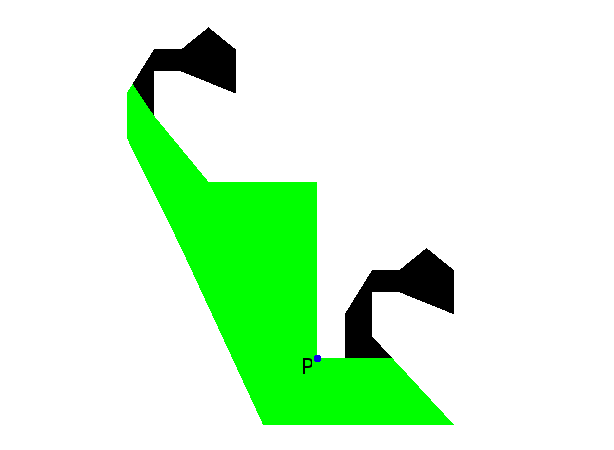
\includegraphics{Images/VisibilityPolygonBird.png}}
\caption{\label{fig:Visibility Polygon of Point}Visibility Polygon of Point}
\end{center}
\end{figure}


\begin{figure}[h]
\begin{center}
\scalebox{0.40}{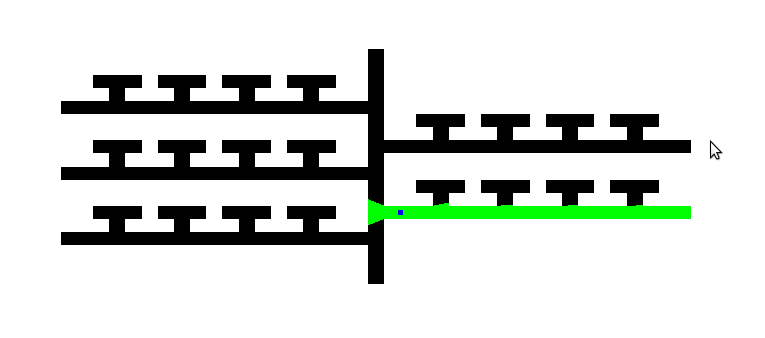
\includegraphics{Images/VisibilityPointOffice.png}}
\caption{\label{fig:Visibility Polygon of Point}Visibility Polygon of Point}
\end{center}
\end{figure}









\subsection{Visibility Polygon of an edge of the polygon}
\begin{definition}
 {\bf Visibility Polygon of Edge:} $e$ is the bounded polygonal region of all points of the polygon visible from any point on the edge $e$. 
\end{definition}

The algorithm for the visibility polygon of an edge has been taken from \cite{key3}.
Let $E$ be the set of edges of the polygon. To find the visibility polygon of an edge $AB$, we compute, for each of 
 the remaining edges of the polygon the portion of it which is weakly visible from the edge $AB$. Once we obtain these portions we join
 all of them to obtain the visibility polygon of the edge $AB$.
  Implementation of this algorithm requires computing shortest path between vertices of the polygon, the construction of which we 
describe in the next section. For now assume that we have at our disposal a routine which gives the shortest path between two vertices 
of the polygon as a list of Point type.

The main steps of computing the visible portion of an edge $CD$ from another edge $AB$ of the polygon can be enumerated as follows.

{\bf Algorithm}



\begin{enumerate}
\item
Compute the shortest path $P_{AC}$, from A to C and the shortest path $P_{BD}$, from B to D. Call this pair 1.
\item
Similarly compute the shortest path  $P_{AD}$, from A to D and the shortest path  $P_{BC}$,  from B to C. Call this pair 2.
\item
Find out which of these pairs is outward convex. An outward convex pair implies an hourglass shape is formed by the two paths.
\item
If none of the pairs is outward convex this means that no portion of edge $CD$ is visible from any point on edge $AB$ and we can 
completely ignore such an edge.

\begin{figure}[h]
\begin{center}
\scalebox{0.50}{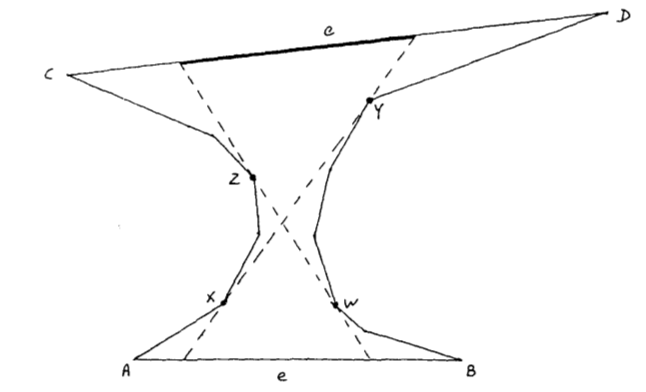
\includegraphics{Images/Cusp.png}}
\caption{\label{fig:Visibility Polygon of Edge}Visibility Polygon of Edge, Illustration taken from:\cite{key3}}
\end{center}
\end{figure}

\item
If one of the pairs is outward convex then without loss of generality, let pair 1 be the outward convex pair. Now compute the shortest 
paths  $P_{AD}$ and  $P_{BC}$.

\item
Let $X$ be the point where path $P_{AD}$ and $P_{AC}$ split and let  $W$ be the point where path $P_{BD}$ and $P_{BC}$ split. Let $Y$ be
the next point on the path  $P_{AD}$ and $Z$ be the next point on the path   $P_{BC}$. Extending $XY$ we get one extreme point of the 
portion of $CD$ visible from $AB$. We repeat this on other side to get the other extreme point.


\end{enumerate}

 $CalcVisibilityPolygonEdge()$ calculates the visibility polygon of an edge in PolygonUtil.cpp

{\bf Note:}
This routine computes the visibility polygon of the edge excluding its endpoints. To obtain the visibility polygon of the edge where
endpoints are inclusive one could compute the visibility polygon of point at the two endpoints and take a union with the visibility
polygon returned by this routine.




\subsection{Shortest Path Calculation}
For the calculation of shortest path between any two vertices of the polygon the following property was exploited.
\begin{itemize}
 \item The shortest path must turn only at vertices of the polygon.
 \item It is possible to move from one vertex to the another only if they are visible to each other.
\end{itemize}

\begin{definition}
{\bf Visibility Graph}The visibility graph of a polygon can be formed as follows. Draw a vertex corresponding to each vertex in the 
polygon. Draw an edge between two vertices if the line joining the corresponding vertices in the polygon lies completely inside the 
polygon.
\end{definition}

For Example \\

\begin{figure}
\begin{center}
\scalebox{0.6}{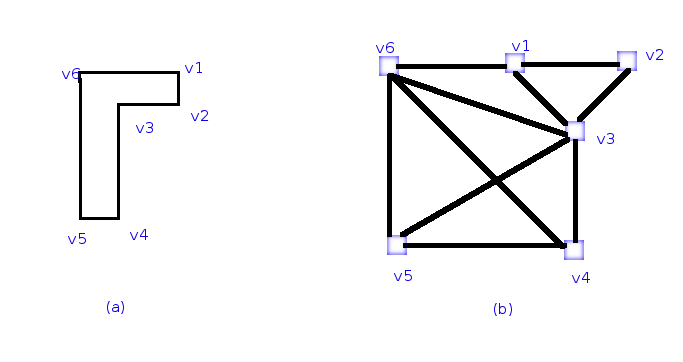
\includegraphics{Images/visibilitygraph.png}}
\caption{\label{fig:Construction} Visibility Graph}
\end{center}
\end{figure}

Utilizing these properties we construct a visibility graph for the polygon and use the normal dijikstra's single source shortest path
algorithm of Boost Graph Libraray \cite{BOOST} on the visibility graph obtained. The following two functions do the above mentioned tasks.



\begin{itemize}


\item
%Java2TeX style definitions
%You can modify them to fit your needs

%%%%%%%%%%%%%%%%%%%%%%%%%%%%%%%%%%%%%%%%%%%%%%%%%%%%%%%%%%%%%%%
%  Java Sourcecode to TeX automatically converted code
%  Java2Html Converter 5.0 [2006-02-26]by Markus Gebhard  markus@jave.de
%     Further information: http://www.java2html.de
{
\noindent \ttfamily
\noindent \ttfamily
\noindent \ttfamily
\noindent \ttfamily
\jttstylek PolygonUtil::PrepareVisibilityGraph\jttstylei (\jttstylek Polygon\&~map,~Point~vertex\jttstylei [])\\

}


\item
%Java2TeX style definitions
%You can modify them to fit your needs

%%%%%%%%%%%%%%%%%%%%%%%%%%%%%%%%%%%%%%%%%%%%%%%%%%%%%%%%%%%%%%%
%  Java Sourcecode to TeX automatically converted code
%  Java2Html Converter 5.0 [2006-02-26]by Markus Gebhard  markus@jave.de
%     Further information: http://www.java2html.de
{
\noindent \ttfamily
\jttstylek PolygonUtil::CalcShortestPath\jttstylei (\jttstylej int~\jttstylek source,graph\verb#_#t\&~g,Point~vertex\jttstylei [])\\
\noindent \ttfamily
}

\end{itemize}

{\bf Examples}

The edge is shown in blue and its visibility polygon is shown in green.

\begin{figure}[h]
\begin{center}
\scalebox{0.50}{
\includegraphics{Images/VisibilityLine1.png}}
\caption{\label{fig:Visibility Polygon of Edge}Visibility Polygon of Edge}
\end{center}
\end{figure}

\begin{figure}[h]
\begin{center}
\scalebox{0.40}{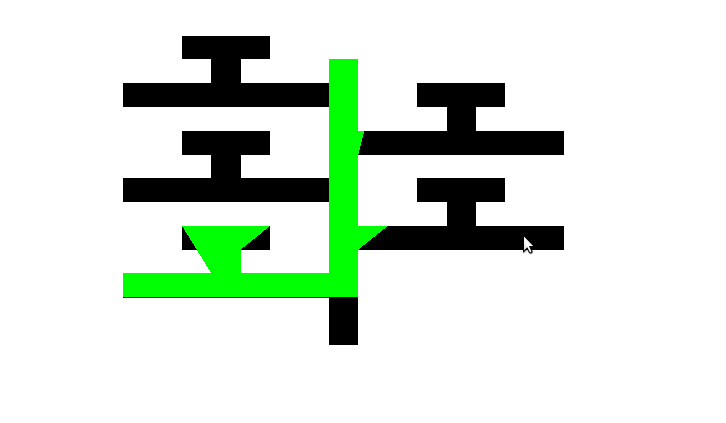
\includegraphics{Images/VisibilityLine2.png}}
\caption{\label{fig:Visibility Polygon of Edge}Visibility Polygon of Edge}
\end{center}
\end{figure}




% ------------------------------------------------------------------------


%%% Local Variables: 
%%% mode: latex
%%% TeX-master: "../thesis"
%%% End: 
